\documentclass[12pt,lettersize]{article}
\usepackage{amsmath}
\usepackage{amsfonts}
\usepackage{xargs}
\usepackage{color}
\usepackage{amssymb}
\usepackage{graphicx}
\usepackage{listings}
\usepackage{tabu}
\usepackage{hyperref}
\usepackage{todonotes}

\newcommandx{\lef}[2][1=]{\todo[linecolor=red,backgroundcolor=red!25,bordercolor=red,size=\footnotesize,#1]{LEF: #2}}
\newcommand{\mwand}{\mathrel{-\mkern-6mu*}}
\newcommand{\valid}[1]{\texttt{valid}\ #1}

\usepackage{listings,lstlangcoq}
\lstdefinestyle{coq}{
  columns=flexible,
  mathescape=true,
  belowcaptionskip=1\baselineskip,
  breaklines=true,
  xleftmargin=0pt,
  language=Coq,
  morekeywords={Variant, fun, Arguments, Type, cofix},
  % morekeywords={SOCKAPI,ITREE,data_at,data_at_},
  emph={%
    SOCKAPI,ITree,CTree,data_at,data_at_
  },
  emphstyle={\bfseries\color{green!40!red!80}},
  showstringspaces=false,
  basicstyle=\small\ttfamily,
  keywordstyle=\bfseries\color{green!20!black},
  commentstyle=\itshape\color{red!40!black},
  identifierstyle=\color{violet!50!black},
  stringstyle=\color{orange},
  escapeinside={<@}{@>}
}
\newcommand{\inlinecoq}[1]{\mbox{\lstinline[style=coq,columns=fixed,basewidth=.48em]{#1}}}


\title{Report: Automated simplification tactics over separation algebras.}
\author{Lef Ioannidis, Yiyun Liu}
\date{\today}

\begin{document}
\maketitle

\begin{abstract}
This report documents the development of an automated simplification tactic for Separation Logic in Coq's Ltac2, based on 
Labeled Sequents of Propositional Abstract Separation Logic (LSPASL)~\cite{hou2017proof}. LSPASL is a labeled sequent calculus
for Abstract Separation Logic based on Separation Algebras ~\cite{calcagno2007local} that we prove sound. Our tactic works for 
a variety of effects, without having to redefine the proof search and simplification for each one. We demonstrate the generality of LSPASL
by instantiating a Heap Separation algebra and the effectiveness with several examples of autoated simplification.
In comparison to \texttt{xsimpl} for Separation Logic Foundations ~\cite{chargueraud2020separation}
our approach is more structured and more general and shows potential for adoption. Our coq development is open source and available
online~\cite{github}.
\end{abstract}

\section{Background and Motivation}
Separation logic significantly simplifies reasoning about programs that manipulate heap-allocated memory, offering a framework
to ensure the correctness of these operations. The tactics introduced in "Separation Logic Foundations"~\cite{chargueraud2020separation}
are especially effective, although their implementation is "fairly involved", according to their author. The \texttt{xsimpl} tactic
for automatically solving assertions is particularly ad-hoc, defined as a functor over many separation logic primitives and laws,
making it cumbersome to initialize.

A more structured and general altenative by Hou et al~\cite{hou2017proof} for Isabelle/HOL, provides powerful automated reasoning
capabilities within Separation Logics. Adapting these tactics for Coq's Ltac2 language can greatly enhance the separation logic verification process in Coq.
By abstracting these tactics over SAs~\cite{calcagno2007local} we aim to offer
flexible tactics that can be applied to programs with ghost state, permissions~\cite{bornat2005permission}, 
histories~\cite{sergey2015specifying} and more.

\section{Design and Implementation}

Our first goal is generality, by using Separation Algebras (SA) to describe arbitrary disjoint effects. In the literature several equivalent definitions appear.
We chose a slightly different definition from Calcagno et al~\cite{calcagno2007local}, they define $+: \Sigma \to \Sigma \to \Sigma$ (pronounced \emph{join})
as a partial, commutative, associative, cancellative binary relation and check validity with the \emph{disjoint} relation $\#: \Sigma \to \Sigma \to \mathbb{P}$.

\subsection{Separation Algebra}
We instead opt for a total join and unary predicate. Here's our formal definition of Separation Algebra, 
a tuple $(\Sigma, +, \texttt{valid}, 0)$ where 

\begin{itemize}
\item $\Sigma$ is the carrier set.
\item $+$ is a binary \emph{total} function over $\Sigma$.
\item $\texttt{valid}$ is a predicate over $\Sigma$.
\item $0$ is the unity of $+$.
\end{itemize}

Our join ($+$) operator is total, commutative, associative and cancellative, with unit element $0$ (pronounced empty) and our $\texttt{valid}$ predicate decides
which states are acceptable. \\

\begin{minipage}{0.8\textwidth}
\begin{flalign*}
&\forall\ a\ b,\ a + b = b + a && (\text{Commutativity}) \\
&\forall\ a\ b\ c,\ (a + b) + c = a + (b + c) && (\text{Associativity}) \\
&\forall\ a,\ a + 0 = a && (\text{Identity-left}) \\
&\valid{0} && (\text{Valid unit}) \\
&\forall\ a\ b,\ \valid{(a + b)} \to \valid{a} && (\text{Valid-left})\\
&\forall\ a\ b\ c,\ \valid{(a + c)} \to a + c = b + c \to a = b && (\text{Cancel-left})\\
\end{flalign*}
\end{minipage}

\subsection{Heaps}
To demonstrate the usuability of our SA definition we instantiate it for a finite heap model. This is one possible way to do the instantiation and not the only one.

Finiteness is required by $\texttt{FMap.disjoin\_union}: FMap\ a\ b \to FMap\ a\ b \to FMap\ a\ b$ in Coq and the outer $\texttt{option}$ is necessary to internalize
the result of an erroneous \emph{join} until it can be checked by $\texttt{valid}$. \\

\begin{minipage}{0.5\textwidth}
\begin{flalign*}
&\Sigma && \triangleq \ \texttt{option } (\texttt{fmap } \mathbb{Z}\ \mathbb{Z}).\\
&a + b && \triangleq \ a \texttt{ >>= } (\lambda a.\ b \texttt{ >>= } (\lambda b. \\
    & && \hspace{2cm} \texttt{FMap.disjoint\_union } a\ b)). \\
&\valid{a} && \triangleq \ \texttt{is\_some }a.\\
&0 && \triangleq \ \texttt{Some }(\lambda x.\ \texttt{None})
\end{flalign*}
\end{minipage}

\vspace*{.2cm}

We additionally must prove the SA axioms, which we did in the Coq development, for exposition we provide the proof sketches for the last two lemmas, 
\emph{Valid-left} and \emph{Cancel-left}, which are the most interesting.

\noindent \textbf{Proof sketch} for $\forall\ a\ b,\ \valid{(a + b)} \to \valid{a}$.\\
By definition of $\texttt{bind}$ in $+$, both arguments in $a + b$ must be $\texttt{Some}$. \\
\noindent \textbf{Proof sketch} for $\forall\ a\ b\ c,\ \valid{(a + c)} \to a + c = b + c \to a = b$. \\
First, use \emph{Valid-left}, \emph{Comm} to show $\texttt{valid }c$. Then, by induction on finite $c$ \\
and cases on $a,\ b$.

\subsection{PASL}
We now build a semantic logical reasoning framework based on SA, the Propositional Abstract Separation Logic (PASL)~\cite{hou2017proof}, based
on Kripke semantics. A Kripke frame for PASL is $\mathcal{M} = (\Sigma, +, \texttt{valid}, 0, v)$ where $v: Var \to \mathcal{P}(\Sigma)$.

\begin{flalign*}
    &\mathcal{M}, \sigma && \vDash p &&\iff \valid{\sigma} \text{ and } \sigma \in v(p) \\
    &\mathcal{M}, \sigma && \vDash \top && \text{ always }\\
    &\mathcal{M}, \sigma && \vDash \bot && \text{ never }\\
    &\mathcal{M}, \sigma && \vDash A \land B &&\iff 
        \mathcal{M}, \sigma \vDash A \text{ and } 
        \mathcal{M}, \sigma \vDash B \\
    &\mathcal{M}, \sigma && \vDash A \lor B &&\iff 
        \mathcal{M}, \sigma \vDash A \text{ or } 
        \mathcal{M}, \sigma \vDash B \\
    &\mathcal{M}, \sigma && \vDash \lnot A &&\iff 
        \mathcal{M}, \sigma \not\vDash A \\
    &\mathcal{M}, \sigma && \vDash A \to B &&\iff 
        \mathcal{M}, \sigma \vDash A \to \mathcal{M}, \sigma \vDash B \\
    &\mathcal{M}, \sigma && \vDash \top^* && \iff h = 0 \\
    &\mathcal{M}, \sigma && \vDash A * B && \iff 
        \exists\ a\ b,\ \sigma = a + b\text{ and }
        \valid{\sigma} \text{ and }
        \mathcal{M}, a \vDash A \text{ and } 
        \mathcal{M}, b \vDash B \\
    &\mathcal{M}, \sigma && \vDash A \mwand B && \iff
        \forall\ a\ b,\ b = \sigma + a \to 
        \valid{\sigma} \to
        \mathcal{M}, a \vDash A \to
        \mathcal{M}, b \vDash B \\
\end{flalign*}

\subsection{LSPASL}

PASL is a semantic framework, for proof-automation a syntactic framework for manipulating PASL formulas and proofs is required.
That is the purpose of the Labeled Sequent PASL (LSPASL). We introduce a set of labels $\mathcal{L} = LVar \cup \{\epsilon\}$ and annotate each PASL formula
with a label $(a:\ A)$, where $a \in \mathcal{L}$ and $A$ is a PASL formula.

In addition, we extend the sequent calculus with a ternary relation on labels $(x, y \triangleright z)\ \triangleq\ \valid{z} \land x + y = z$.
Now we can give the formal definition of a LSPASL sequent, based on Kripke frames.

An extended Kripke frame for LSPASL is $\mathcal{M} = (\Sigma, +, \texttt{valid}, 0, v, \mathcal{L}, \rho)$ where
labels $\mathcal{L}\ \triangleq \ LVar \cup \{ \epsilon \}$ and
label valuation function $\rho: \mathcal{L} \to \Sigma$. \\

\noindent A sequent $G, \Gamma \vdash \Delta$ iff
\begin{itemize}
\item $\forall\ (x: A) \in \Gamma,\ (y: B) \in \Delta$.
\item $\forall (a, b \triangleright c) \in G$.
\item $\mathcal{M}, \rho(x) \vDash A$ and
      $\rho(a) + \rho(b) = \rho(c)$ and $\valid{\rho(c)}$ and
      $\mathcal{M}, \rho(y) \vDash(B) $.
\end{itemize}

Now we can prove the syntactic lemmas of LSPASL which are used during proof search, from the above semantic definition using the extended Kripke frame.

\begin{figure}
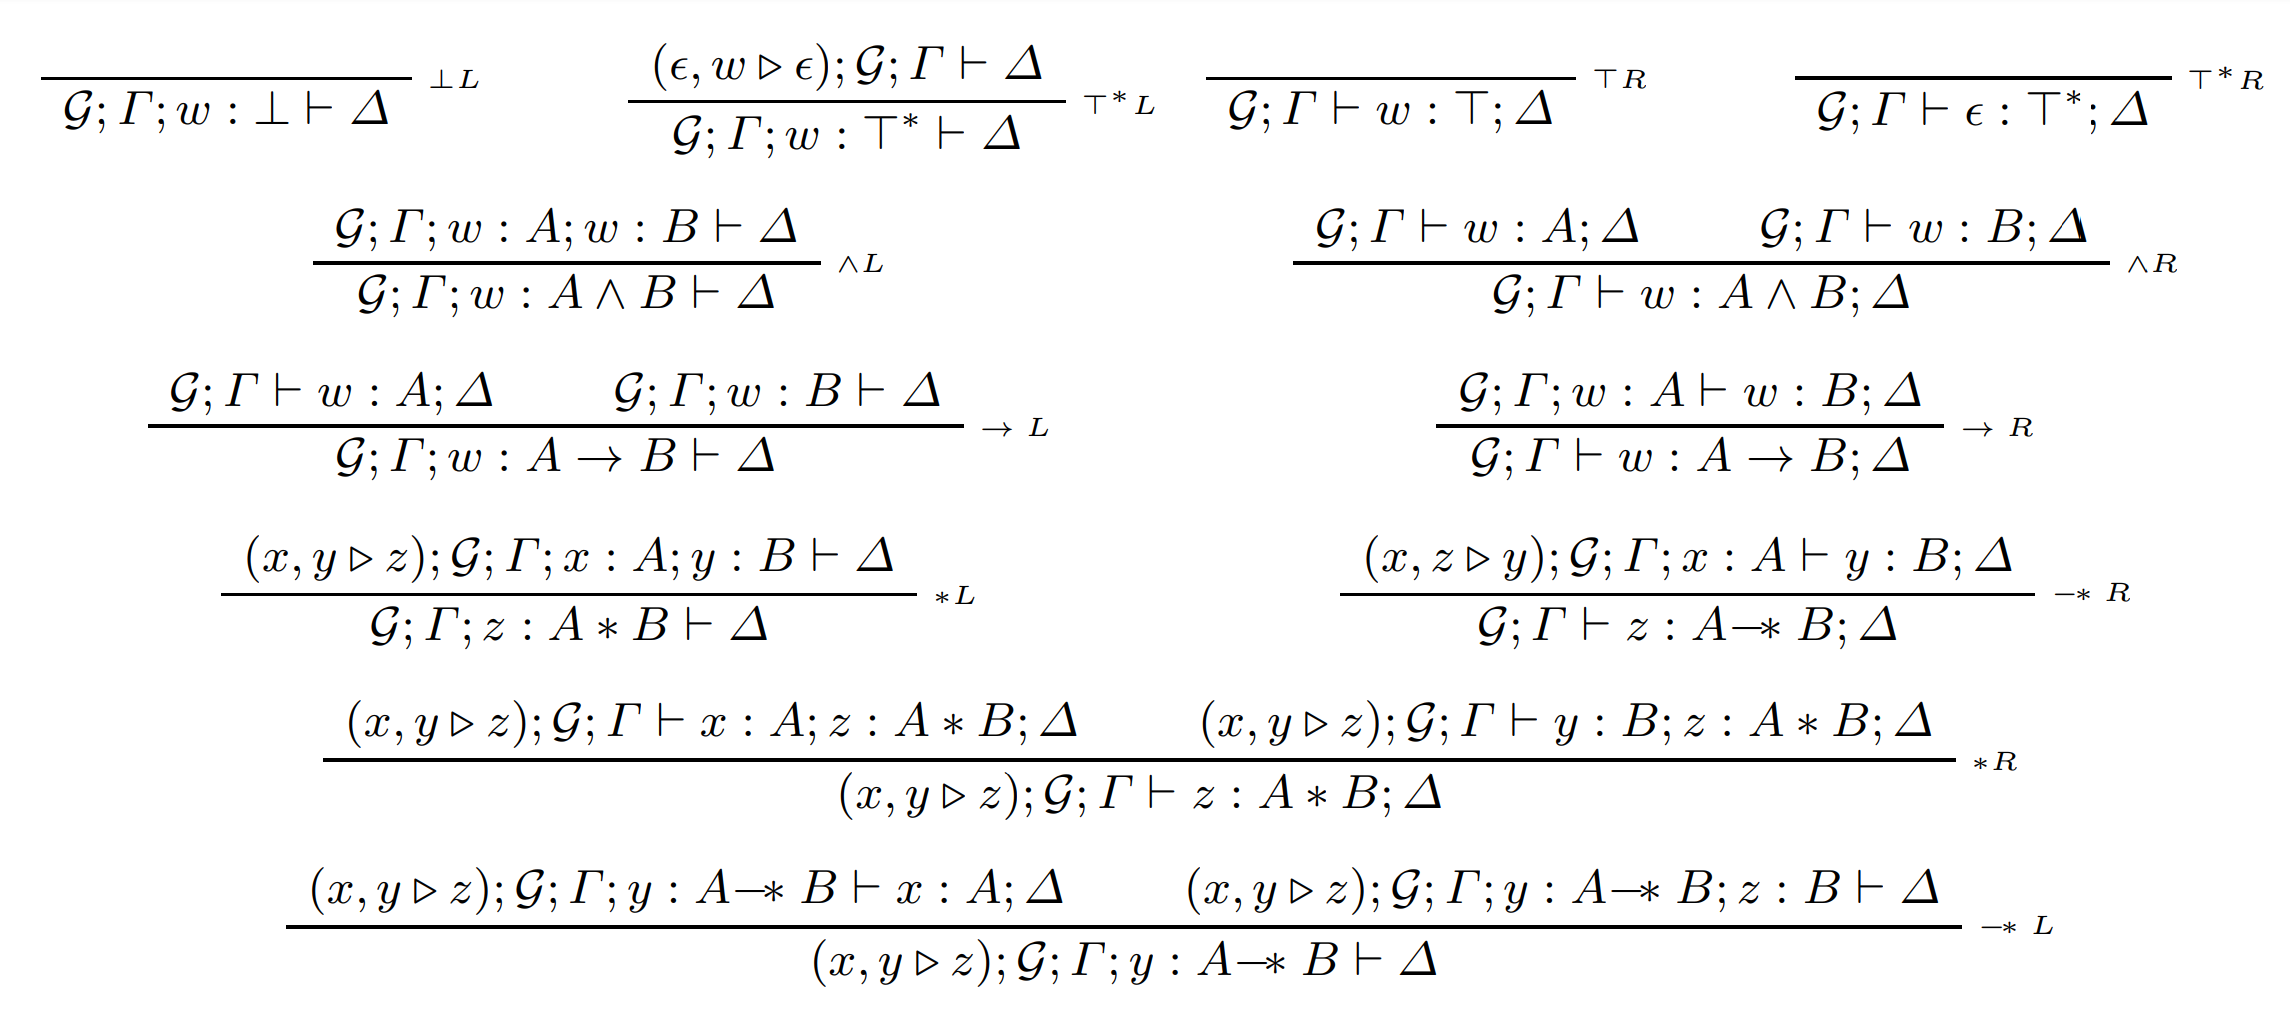
\includegraphics[width=\textwidth]{LSPASLtrans.png}
\caption{The labelled sequent calculus LSPASL for Propositional Abstract Separation Logic, defined by H\'{o}u et al~\cite{hou2017proof}.}
\label{fig:lspasl}
\end{figure}

We proved the syntatic rules in fig.~\ref{fig:lspasl} in Coq and also proved soundness, meaning the syntactic rules follow from the semantic definition
of LSPASL satisfiability.
$$ \forall\ \mathcal{G} \ \Gamma\ \Delta, \ \mathcal{G},\ \Gamma \vdash \Delta  \to  \mathcal{G},\ \Gamma \vDash \Delta $$

\section{Reify tactic}

Using the soundness lemma we prove the \emph{transform\_sound} lemma in Coq. We can use this lemma to transform a goal from
its semantic representation into it's syntactic representation, where it is amenable to proof search.
\begin{lstlisting}[style=coq]
Lemma transform_sound (a : Exp) (A : Assertion) :
    valid (denoteExp a) ->
    expToRelAtoms a ;; nil |- ((denoteExp a , A) :: nil) ->
    denoteExp a \in denoteAssertion A.
\end{lstlisting}

This is the core of our $\texttt{reify}$ tactic, as a series of steps
\begin{itemize}
\item Refify the goal using $\texttt{transform\_sound}$.
\item Using $\texttt{eauto using lspasl}$ with the LSPASL lemmas of fig.~\ref{fig:lspasl}, apply any number of constructors until the goal is proved.
\end{itemize}

\section{Examples}
We prove the following examples in a semi-automated way using the \emph{reify} tactic. One issue is our use of $\texttt{list}$ for representing
sequent contexts, is not able to recognize equality of lists up-to-permutation. Some manual interventention is needed to show two
contexts are indeed permutations of each other. In the paper, they used \emph{multisets} which would not require this.

\begin{figure}
\begin{lstlisting}[style=coq]
Lemma ex1 : unit \in semp.
Lemma ex2 : unit \+ unit \in sstar semp semp.
Lemma ex3 (a b : T) (A B : T -> Prop) :
    valid (a \+ b) ->
    a \+ b \in simp (sstar A B) (sstar B A).
\end{lstlisting}
\caption{Three examples we were able to prove using the \emph{reify} tactic.}
\label{fig:examples}
\end{figure}

We show the examples we proved in our development in fig.~\ref{fig:examples}.

\section{Future work}
In this work and in the interest of time we did not show \emph{completeness}.
As a result, we can prove goals but cannot syntactically manipulate sequents in Coq's proof context. We believe
completeness is more involved and requires an intermediate extension to LSPASL~\cite{hou2017proof}. 

In addition, using multisets to represent sequents would allow us to reason seamlessly up-to-permutation, without the need for user intervention.
Finally, we would like to see a variant of this automation procedure integrated in a Separation Logic framework like Iris~\cite{jung2018iris} or CN~\cite{pulte2023cn}.

\bibliographystyle{plain}
\bibliography{main}

\end{document}
